\documentclass[11pt,letter]{article}

\usepackage[portuguese]{babel}
\usepackage{biblatex}
\usepackage[utf8]{inputenc}
\usepackage{csquotes}
\usepackage[T1]{fontenc}
\usepackage{charter}
\usepackage{graphicx}
\usepackage{caption}
\usepackage{float}
\usepackage{amsmath}
\usepackage{tabularx}
\usepackage{multirow}
\usepackage{textcomp}
\usepackage{multicol}
\usepackage{setspace}
\usepackage{geometry}
\usepackage{indentfirst}
\usepackage{verbatim}
\geometry{top=2cm,bottom=2cm,left=2cm,right=2cm}

\usepackage{hyperref}

\graphicspath{ {fig/} }
\addbibresource{ref.bib}

\newenvironment{myenumerate}{
	\begin{enumerate}
		\setlength{\itemsep}{-2pt}
		\setlength{\parskip}{0pt}
		\setlength{\parsep}{5pt}
	}{\end{enumerate}}

\newenvironment{myitemize}{
	\begin{itemize}
		\setlength{\itemsep}{5pt}
		\setlength{\parskip}{0pt}
		\setlength{\parsep}{5pt}
	}{\end{itemize}}

%\renewcommand{\familydefault}{\sfdefault}

\renewcommand\refname{Referências Bibliográficas}

\begin{document}
	
	\tolerance=999
	\sloppy
	
	\thispagestyle{empty}
	
	\begin{center}
		\rule{\textwidth}{1pt}
	\end{center}
	
	\vspace*{-0.2cm}
	
	\begin{figure}[!ht]
		\begin{minipage}[b]{2.3cm}
			\centering
			\hspace*{0.4cm}
			
\includegraphics[width=2.0cm]{./fig/logo-unicamp-name-line-blk-red-0480-eps-converted-to.pdf}
		\end{minipage}
		\begin{minipage}[b]{11.1cm}
			\centering
			\hspace*{0.4cm}
			{\large \bf Universidade Estadual de Campinas} \\[0.2cm]
			{\large \bf Instituto de Computação}
		\end{minipage}
		\begin{minipage}[b]{2.3cm}
			\centering
			\hspace*{0.4cm}
			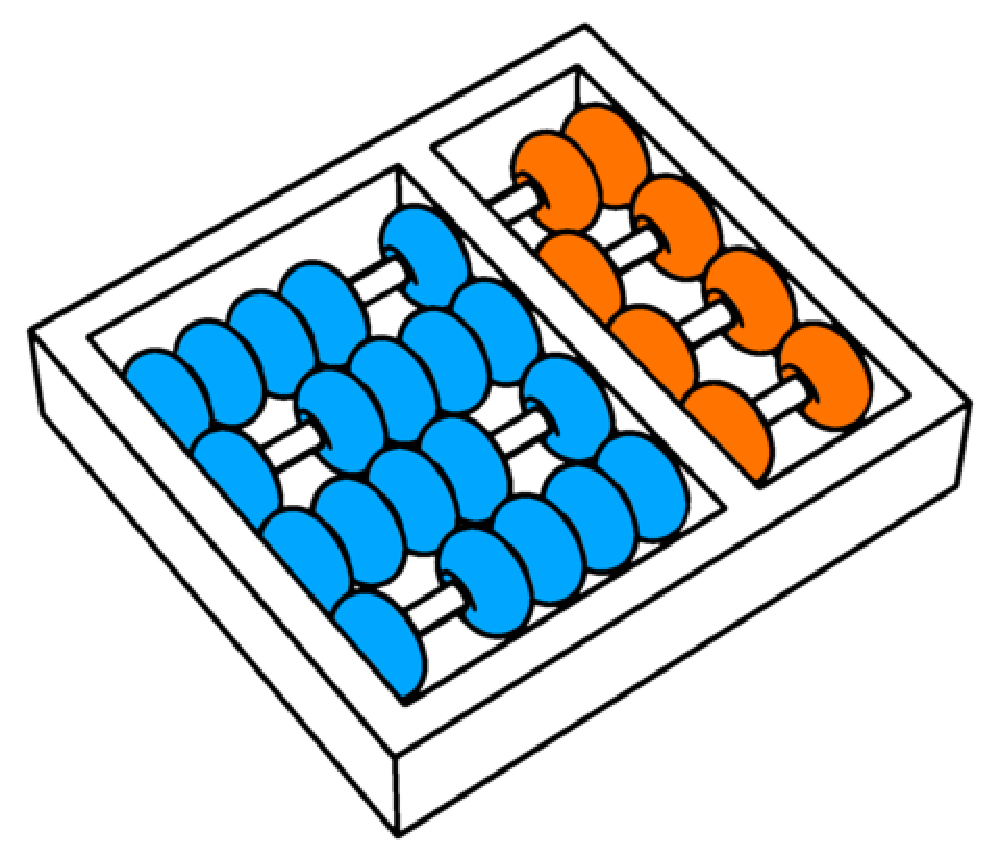
\includegraphics[width=2.0cm]{./fig/logo-ic-unicamp-slant-line-wht-sky-ora-0480-eps-converted-to.pdf}
		\end{minipage}
	\end{figure}
	
	\vspace*{-0.2cm}
	
	\begin{center}
		\rule{\textwidth}{1pt}
	\end{center}
	
	\vspace*{0.1cm}
	
	\begin{spacing}{1.2}
		\begin{center}
			{\Large \bf MO434 - Deep Learning}
			\\ [0.5cm]
		\end{center}
	\end{spacing}
	
	\begin{spacing}{1.3}
		\pagenumbering{arabic}
		\setcounter{page}{1}
		\noindent \textbf{Identificação}: Christian Massao Konishi -- RA 214570\\
		\abstract{
Inserir resumo
}
		\vspace*{\fill}
		
		\centerline{\today}
		
		\newpage
		
		\section{Exercício 1 -- Exemplo de uma primeira rede neural para imagens}

\begin{itemize}
	\item Notebook: \textit{first-image-neuralnet.ipynb}
\end{itemize}

\subsection{Descrição}
		\section{Exercício 2 -- Introdução ao Pytorch Convnet}

\begin{itemize}
	\item Notebook: \textit{introducing-pytorch-convnet.ipynb}
\end{itemize}

\subsection{Descrição}

O notebook em questão contém uma série de demonstrações de conceitos básicos do Pytorch, como as operações de convolução, a função de ativação, \textit{pooling}. Além de \textit{skip connections}, camadas densamente conectadas, \textit{dropout} etc. Por fim, há um processo de construção e treinamento de uma rede neural, desde sua construção, definição de função de perda e otimizador, processo de treinamento e validação.

O problema do processo que foi realizado é que houve \textit{overfitting}. O exercício em questão consiste numa exploração dos elementos e hiperparâmetros utilizados para melhorar o resultado obtido

\subsection{Conceitos}
		
		\printbibliography 
	\end{spacing}
	
	\vfill
	
\end{document}
